\documentclass[a4paper,12pt]{article}
\usepackage{sectsty}
\setlength{\oddsidemargin}{0in}
\setlength{\evensidemargin}{0in}
\setlength{\textwidth}{6.75in}
\setlength{\topmargin}{-0.5in}
\setlength{\textheight}{9.25in}
\setlength{\parindent}{0pt}

\usepackage{fancyhdr}
\usepackage{graphicx}
\usepackage{float}
\graphicspath{ {./figs/} }
\usepackage[ruled,vlined]{algorithm2e}
\usepackage{hyperref}
\hypersetup{
    colorlinks=true,
    linkcolor=blue,
    filecolor=magenta,      
    urlcolor=cyan,
}
\sectionfont{\normalsize}
 
\pagestyle{fancy}
\fancyhf{}
\lhead{CS 532 : Project 1}
\rhead{Group 3}

\usepackage{dirtytalk}
\usepackage{amssymb}
\usepackage{amsfonts}
\usepackage{amsmath}

\sectionfont{\normalsize}

%adjusting the font size for section headings
\usepackage{titlesec}
\titleformat*{\section}{\Large\bfseries}
\titleformat*{\subsection}{\large\bfseries}
\titleformat*{\subsubsection}{\large\bfseries}
\titleformat*{\paragraph}{\largeseries}
\titleformat*{\subparagraph}{\large\bfseries}


\title{%
\textbf{COMPSCI 532: MapReduce}\\
\large \textit{\textbf{Technical Design Document}}}
\author{Dhruv Agarwal (dagarwal@umass.edu)\\
Shantam Shorewala (sshorewala@umass.edu)\\
Shubham Shetty (shubhamshett@umass.edu)}
\date{\textit{March 2021}}

\begin{document}

    \begin{titlepage}
        \maketitle
        \thispagestyle{empty}
    \end{titlepage}

\newpage

\setcounter{page}{1}
\pagenumbering{arabic}
\cfoot{\thepage}

\section{Introduction}
In this project we have implemented a basic version of MapReduce running on a single server with multiprocessing and fault tolerance. MapReduce is a programming model developed to deal with processing large datasets in an efficient and easily parallelizable manner. The core components behind MapReduce are the master and the workers (Mappers or Reducers) - Master process controls the execution flow, while Mappers and Reducers execute the functions on the data.

\subsection{Project Overview}
The main objective of the project is to create a library which provides the end-user the ability to write MapReduce jobs without having to worry about technical details such as file partitioning, parallelization, or multiprocessing. The user can utilize the library to write custom functions (User Defined Functions or UDFs) which follow the MapReduce framework to process large amounts of data.\\

The user provides a config file which contains details such as the location of an input file, the location of the output files, number of mappers/reducers, etc. The user then defines custom mapper and reducer functions using the MapReduce library and then runs the program. The program invokes the MapReduce class, which in turn internally partitions the input file and distributes the data across mapper processes. After completion of Mapper processes, the master then invokes the reducer workers which use the intermediate data as input. The worker processes are executed in parallel with the master process only managing the execution flow. Additionally, the master provides fault tolerance by constantly checking the workers for heartbeat status, and restarting any process which may have been terminated or timed out. All these functionalities were designed according to the specifications mentioned in the source paper.

\subsection{Technical Requirements}
We have chosen to use Python 3 to develop our library for this project. The project uses \emph{conda} for package, environment, and dependency management via an \textit{environment.yml} file, which tracks the project dependencies, including the Python version against which our system is stable. Following Python libraries were used for our program - 
\begin{itemize}
    \item \textit{os}
    \item \textit{pathlib}
    \item \textit{time}
    \item \textit{multiprocessing}
    \item \textit{collections}
    \item \textit{pickle}
    \item \textit{itertools}
\end{itemize}

\section{System Design}

\subsection{Execution Flow}
    \begin{figure}[H]
        % \centering
        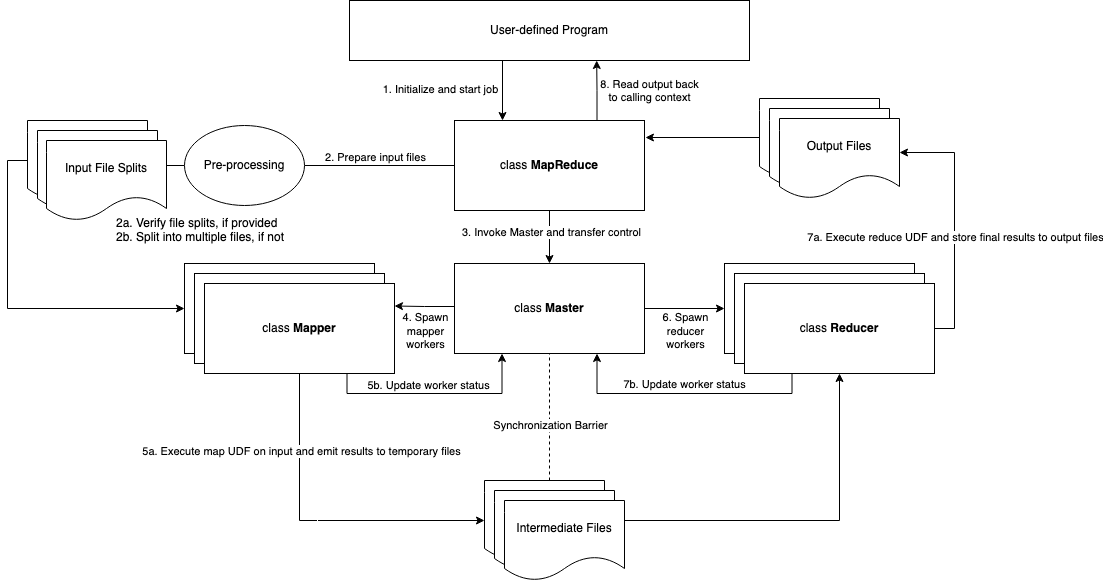
\includegraphics[width=\textwidth]{mapreduce_flow}
        \caption{MapReduce execution flow}
    \end{figure}
The execution of the MapReduce framework (Figure 1) is driven by a user-defined program that creates a job, which is an object of the exposed MapReduce class. After instantiation, the MapReduce class performs pre-processing steps, which are detailed in the following section. The control is then transferred to the Master class, which is responsible for the allocation and execution of workers, in addition to tracking the locations of the intermediate and final output files. \newline

The Master first operates in the "Map Phase" where it spawns and executes M workers (based on the job configuration and input splits) in parallel. Each worker reads its own split of the input data and outputs R intermediate files based on the map UDF. In addition, each iteration of the execution is accompanied by a heartbeat-like status update back to the Master indicating that the worker is still alive. If the Master does not receive a status update from its worker, it assumes a crash and invokes a new worker. \newline

The Master operates with a synchronization barrier, which ensures that all mappers must finish execution before the Master can transition to the "Reduce Phase". In this phase, R reduce workers read the intermediate output files from the mappers, and begin executing a shuffle and reduce operation based on the reduce UDF. Each reduce worker writes one final output file to disk.

\subsection{MapReduce (Class)}
The MapReduce class is the container class for the framework that allows a user program to create a job and retrieve the results. In order to create a job, a program must specify the number of mappers, number of reducers, the path to the input file or directory, the map UDF (user-defined function), and the reduce UDF. \newline

Before Master invocation, the class first executes a few pre-processing steps to prepare the job. First, the server's CPU count is checked to upper-bound the user's configuration for the number of mappers and reducers. Next, the paths to the intermediate and final output directories are tracked and the directories are created. Then, \textit{input\_path} is evaluated to verify compatibility. If the user passed a directory path, the class verifies if at least one file is found within it or not, and if the number of files found are less than the number of mappers configured, the configuration is lowered to the file count. If the user passed a file path, the class reads the file line by line and splits it into multiple files based on the number of mappers configured. \newline

Once pre-processed, the MapReduce class invokes the Master and begins execution.

\subsection{Master}

\begin{itemize}
    \item The Master class, on instantiation, takes as argument the number of mappers and reducers, path to the input files as well as the disk location for temporary and output files. Using the CPU count, master determines the optimal number of mappers/reducers to spawn (minimum of CPU count and user-defined number of mappers/reducers). Hence, the setup can be considered as a multi-server system with one process running per system.
    \item When the Master is spawned, it first instantiates M mappers -- each running as an isolated process. For each mapper, a duplex channel is setup for message passing using a queue data structure. Master starts all the processes and periodically listens for the status message from each mapper. When all the mappers return a message with status DONE, Master concludes the Map phase. Mapper workers are also responsible for sharing the keys that they have operated upon with the Master.
    \item Master then starts the Reduce phase by initiating R reducers and sharing the location of intermediate files with the reducer workers as well as the keys encountered in Map phase. Similar to Map phase, each reducer can pass messages to the Master via a queue. Master waits until all the reducer workers return a message indicating that they have successfully finished executing. 
    \item Fault tolerance: While checking for heartbeat messages regarding worker's status, Master waits for a fixed time interval. If the worker does not respond within this period, Master assumes that the worker is either dead or is unable to progress due to a lack of resources. In either case, Master then executes a sequence to kill the unresponsive worker and spawn a replacement process to complete the task. Further, Master also tracks the number of reattempts for each input/intermediate split and aborts the task if it exceeds the maximum amount of attempts allowed.
    
\end{itemize}

\subsection{Mapper}
Each Mapper worker is instantiated with an ID, the number of reducers for the job, the path to its input file partition, the intermediate output path, and the map UDF. The execution begins with the mapper reading the data from its partition and changing its status to `RUNNING'. For each line in the partition file, the mapper executes the UDF and emits an intermediate (key,value) pair to a reducer ID that is determined by taking a modulo of the hash of the key with the number of reducers configured for the job. These values are stored in a dict structure keyed on reducer IDs, which in turn hold dicts that are keyed on the emitted key names. Once all lines are read and processed, the mapper stores the intermediate results to R number of pickle files containing data pertaining to each reducer. The mapper then changes its status to `DONE' and sends this update back to the Master.

\subsection{Reducer}
Once all mappers complete execution and update status to `DONE', the Master process can move on to the Reduce phase. Similar to the Map phase, the Master first instantiates each Reducer worker with an id, number of mappers for the job, path to the intermediate files, an output file path, and the reducer UDF. Each reducer worker process reads its corresponding intermediate file and updates its status to `RUNNING'. Once a reducer worker reads the key-value pairs from the intermediate file, it executes the UDF reducer on the data. Once final output is generated, each worker then writes it to the final output path and updates status to `DONE' before returning control to the master.

\section{System Considerations/Evaluation}

\begin{itemize}
    \item Message passing: Since we use Python 3, our implementation involves using multiple processes and not threads (due to the Global Interpreter Lock). Hence, all communication is handled using message passing which simulates a distributed system (no shared memory). 
    \item In addition to writing one output file per reducer worker, MapReduce also aggregates the data from all the output files as a key-value list in order to share it with the user program. This design choice is made to ensure that if the output is needed for any reason (such as cascaded MapReduce jobs), the user program does not need to fetch the output data from disk, minimizing read-write overhead.
    \item Fault tolerance is incorporated keeping in mind different types of failures -- process (and hence, server) crash or lack of resources (stragglers). Keeping this in mind, the Master interprets missing heartbeat messages as the condition for a timeout rather than explicitly only checking whether is a process is alive or dead.
    \item System is evaluated using a variety of test cases as well as edge cases resulting in faults to determine how robust the system's fault tolerance is. System is able to successfully detect faulty workers and respawn replacements to complete the task in a reasonable time period. The system is able to handle multiple faulty workers for the same task, only constrained by the number of reattempts per split before aborting a task.
    
\end{itemize}

\section{Test Cases}

\subsection{Word Count \textbf{(with fault tolerance)}}
Program to read a text file containing 5900 lines and count the number of occurrences of each unique word in the file, where the split of words is based on a space-character. Additionally, we artificially kill the 3rd mapper and showcase the ability of the framework to recover and spawn a new worker. \newline

\textbf{Test configuration:}
\begin{itemize}
    \item Test file: test\_1.py
    \item Mappers: 10
    \item Reducers: 3
    \item Worker Kill Index: 2 (third worker)
    \item Job config: data/config\_word\_count.txt
    \item Input: data/hamlet.txt
\end{itemize}

\subsection{Average Test Score}
Program that randomly generates 10,000 lines of ``$<$name$>$ $<$score$>$" combinations from a list of pre-defined names and scores ranging from 0 to 100, and computes the average scores for 3 names - Shubham, Dhruv, and Shantam. \newline

\textbf{Test configuration:}
\begin{itemize}
    \item Test file: test\_2.py
    \item Mappers: 5
    \item Reducers: 3
    \item Job config: data/config\_test\_score.txt
    \item Input: data/test\_scores.txt
\end{itemize}

\subsection{K-Nearest Neighbors Search}
Program that randomly generates 10,000 examples of 10-D data points and a randomly generated 10-D query vector, and finds the K nearest neighbors for the query vector for K=4. In addition to the regular operation, this test case showcases the ability to chain MapReduce jobs in order to execute successive map and reduce logic. \newline

\textbf{Test configuration:}
\begin{itemize}
    \item Test file: test\_3.py
    \item Mappers: 5, 5
    \item Reducers: 5, 1
    \item Job config: data/config\_knn.txt
    \item Input: data/knn-dataset.txt
\end{itemize}

\subsection{Word Count \textbf{(with fault tolerance and re-spawn limit)}}
Program to read a text file containing 5900 lines and count the number of occurrences of each unique word in the file, where the split of words is based on a space-character. Additionally, we artificially kill the 2nd mapper and showcase the ability of the framework to recover and spawn a new worker. Further, we show that if the worker continues to fail after multiple re-spawns (3), then the MapReduce job throws an error to the user-program. \newline

\textbf{Test configuration:}
\begin{itemize}
    \item Test file: test\_1.py
    \item Mappers: 10
    \item Reducers: 3
    \item Worker Kill Index: -2 (second worker with repeated failure)
    \item Job config: data/config\_word\_count.txt
    \item Input: data/hamlet.txt
\end{itemize}

\section{References}
\begin{enumerate}
    \item Jeffrey Dean and Sanjay Ghemawat: MapReduce: Simplified Data Processing on Large Clusters (2004) (\nolinkurl{https://research.google/pubs/pub62/})
    \item What Is the Python Global Interpreter Lock (GIL)? (\nolinkurl{https://realpython.com/python-gil/})
    \item StackOverflow: error with module multiprocessing under python3.8 (\nolinkurl{https://stackoverflow.com/a/65666298/2923106})
    \item StackOverflow: Merging Python dictionaries using itertools (\nolinkurl{https://stackoverflow.com/questions/2365921/merging-python-dictionaries})
\end{enumerate}

\end{document}